%%%%%%%%%%%%%%%%%%%%%%%%%%%%%%%%%%%%%%%%%%%
%
% From a template maintained at https://github.com/jamesrobertlloyd/cbl-tikz-poster
%
% Code near the top should be fairly standard and not need to be changed
%  - except for the document class
% Code lower down is more likely to be customised
%
%%%%%%%%%%%%%%%%%%%%%%%%%%%%%%%%%%%%%%%%%%%

%%%%%%%%%%%%%%%%%%%%%%%%%%%%%%%%%%%%%%%%%%%
%
% Document class
%
% Change this if you want a different size / orientation poster etc
%
%%%%%%%%%%%%%%%%%%%%%%%%%%%%%%%%%%%%%%%%%%%

%\documentclass[portrait,a0,final]{a0poster}
\documentclass[landscape,a0b,final]{a0poster}

%%%%%%%%%%%%%%%%%%%%%%%%%%%%%%%%%%%%%%%%%%%
%
% 'Basic' packages
%
% TODO - Almost certainly some are unnecessary - feel free to remove nonstandard
% packages if you think it is a good idea not to always have them
%
%%%%%%%%%%%%%%%%%%%%%%%%%%%%%%%%%%%%%%%%%%%

\usepackage{wrapfig}
\usepackage{multicol}
\usepackage{color}
\usepackage{shadow}
\usepackage{morefloats}
%\usepackage{cite}
\usepackage[pdftex]{graphicx}
\usepackage{rotating}
\usepackage{amsmath, amsthm, amssymb, bm}
\usepackage{array}
\usepackage{nth}
\usepackage[square,numbers]{natbib}
\usepackage{booktabs}
\usepackage[table,xcdraw]{xcolor}
\usepackage{float}
%\usepackage{subfig}
%\usepackage{svg}
%\usepackage{wrapfig}
%\usepackage[a0paper,pass]{geometry}
\usepackage[%
    font={small,sf},
    labelfont=bf,
    format=hang,    
    format=plain,
    margin=0pt,
    width=0.8\textwidth,
]{caption}
\usepackage[list=true]{subcaption}
\usepackage{graphicx,array}
%%%%%%%%%%%%%%%%%%%%%%%%%%%%%%%%%%%%%%%%%%%
%
% TIKZ packages and common definitions
%
% Add extra things as per your tikz needs
%
%%%%%%%%%%%%%%%%%%%%%%%%%%%%%%%%%%%%%%%%%%%

\usepackage{picins}
\usepackage{tikz}
\usetikzlibrary{shapes.geometric,arrows,chains,matrix,positioning,scopes,calc}
\tikzstyle{mybox} = [draw=white, rectangle]

%%%%%%%%%%%%%%%%%%%%%%%%%%%%%%%%%%%%%%%%%%%
%
% myfig
%
% \myfig - replacement for \figure
% necessary, since in multicol-environment 
% \figure won't work        
%                 
%%%%%%%%%%%%%%%%%%%%%%%%%%%%%%%%%%%%%%%%%%%

\newcommand{\myfig}[3][0]{
\begin{center}
  \vspace{1.5cm}
  \includegraphics[width=#3\hsize,angle=#1]{#2}
  \nobreak\medskip
\end{center}}

%%%%%%%%%%%%%%%%%%%%%%%%%%%%%%%%%%%%%%%%%%%
%
% mycaption                
%
% \mycaption - replacement for \caption
% necessary, since in multicol-environment \figure and
% therefore \caption won't work
%
%%%%%%%%%%%%%%%%%%%%%%%%%%%%%%%%%%%%%%%%%%%

%\newcounter{figure}
\setcounter{figure}{1}
\newcommand{\mycaption}[1]{
  \vspace{0.5cm}
  \begin{quote}
    {#1}
  \end{quote}
  \vspace{1cm}
  \stepcounter{figure}
}

\newcommand{\cwicaption}[1]{
  %\vspace{0.5cm}
  \begin{quote}
    {{\sc Figure} \arabic{figure}: #1}
  \end{quote}
  %\vspace{1cm}
  \stepcounter{figure}
}

%%%%%%%%%%%%%%%%%%%%%%%%%%%%%%%%%%%%%%%%%%%
%
% Some standard colours
%
%%%%%%%%%%%%%%%%%%%%%%%%%%%%%%%%%%%%%%%%%%%

\definecolor{camlightblue}{rgb}{0.601 , 0.8, 1}
\definecolor{camdarkblue}{rgb}{0, 0.203, 0.402}
\definecolor{camred}{rgb}{1, 0.203, 0}
\definecolor{camyellow}{rgb}{1, 0.8, 0}
\definecolor{lightblue}{rgb}{0, 0, 0.80}
\definecolor{white}{rgb}{1, 1, 1}
\definecolor{whiteblue}{rgb}{0.80, 0.80, 1}
\definecolor{cwired}{rgb}{0.803,0.0,0.227}

%%%%%%%%%%%%%%%%%%%%%%%%%%%%%%%%%%%%%%%%%%%
%
% Some look and feel definitions
%
%%%%%%%%%%%%%%%%%%%%%%%%%%%%%%%%%%%%%%%%%%%

\setlength{\columnsep}{0.03\textwidth}
\setlength{\columnseprule}{0.0018\textwidth}
\setlength{\parindent}{0.0cm}

%%%%%%%%%%%%%%%%%%%%%%%%%%%%%%%%%%%%%%%%%%%
%
% \mysection - replacement for \section*
% 
% Puts a pretty box around some text
% TODO - any other thoughts for what this box should look like
%
%%%%%%%%%%%%%%%%%%%%%%%%%%%%%%%%%%%%%%%%%%%

\tikzstyle{mysection} = [rectangle, 
						draw=none, 
						shade, 
						outer color=cwired,
						inner color=cwired,
						text width=0.95\columnwidth,
						text centered,
						rounded corners=20pt,
						minimum height=0.11\columnwidth]

\newcommand{\mysection}[1]
{
\begin{center}
  \begin{tikzpicture}
    \node[mysection,white] {\sffamily\bfseries\LARGE#1};
  \end{tikzpicture}
\end{center}
}



%%%%%%%%%%%%%%%%%%%%%%%%%%%%%%%%%%%%%%%%%%%
%
% Set the font
%
% TODO - Not sure what a canonical choice is - feel free to modify
%
%%%%%%%%%%%%%%%%%%%%%%%%%%%%%%%%%%%%%%%%%%%

\renewcommand{\familydefault}{cmss}
\sffamily

%%%%%%%%%%%%%%%%%%%%%%%%%%%%%%%%%%%%%%%%%%%
%
% Poster environment
%
% Centres everything and can be used to define the width of the content
%
%%%%%%%%%%%%%%%%%%%%%%%%%%%%%%%%%%%%%%%%%%%

\newenvironment{poster}{
  \begin{center}
  \begin{minipage}[c]{0.95\textwidth}
}{
  \end{minipage} 
  \end{center}
}

%%%%%%%%%%%%%%%%%%%%%%%%%%%%%%%%%%%%%%%%%%%
%
% This is probably a good place to put content specific packages and definitions
%
%%%%%%%%%%%%%%%%%%%%%%%%%%%%%%%%%%%%%%%%%%%

%%%%%%%%%%%%%%%%%%%%%%%%%%%%%%%%%%%%%%%%%%%
%
% The document environment starts here
%
%%%%%%%%%%%%%%%%%%%%%%%%%%%%%%%%%%%%%%%%%%%

\begin{document}
%%%%%%%%%%%%%%%%%%%%%%%%%%%%%%%%%%%%%%%%%%%
%
% Begin the poster environment - centres things and potentially changes the width
%
%%%%%%%%%%%%%%%%%%%%%%%%%%%%%%%%%%%%%%%%%%%

\begin{poster}

%%%%%%%%%%%%%%%%%%%%%%%%%%%%%%%%%%%%%%%%%%%
%
% Potentially add some space at the top of the poster
%
%%%%%%%%%%%%%%%%%%%%%%%%%%%%%%%%%%%%%%%%%%%

\vspace{1\baselineskip}

%%%%%%%%%%%%%%%%%%%%%%%%%%%%%%%%%%%%%%%%%%%
%
% Draw the header as a TIKZ picture
%
% Using TIKZ to allow for easy alignment
%
%%%%%%%%%%%%%%%%%%%%%%%%%%%%%%%%%%%%%%%%%%%

\begin{center}
\begin{tikzpicture}[x=0.5\textwidth]
    % Dummy nodes at edges for spacing
    % TODO - a better way?
    \node at (+1, 0) {};    
    \node at (-1, 0) {};
    % Set the size of the badges
    \def \badgeheight {0.08\textwidth}
    % Title text
    \node[inner sep=0,text width=0.8\textwidth,text centered,font=\Huge] (Title) at (-0.2,0) 
    {
        {\sffamily\veryHuge \color{cwired} \textbf{Bayesian Inference of Radiation Belt Loss Timescales \\ A Surrogate Model Approach}}\\
        {\sffamily\Huge Mandar Chandorkar$^{1,2}$, \underline{Enrico Camporeale}$^1$}\\
        \vspace{-0.2\baselineskip}
        {\sffamily\LARGE 1 Multiscale Dynamics, CWI, Amsterdam, 2 INRIA Paris-Saclay}\\
        \vspace{-0.3\baselineskip}
        {\sffamily\LARGE \color{cwired} www.mlspaceweather.org}
    };
    % Cambridge badge
    \node [mybox] (CWI Logo) at (-1, -0.4) {
        
\includegraphics[height=0.055\textwidth]{cwi-logo.png}
    };
    % CBL badge
    \node [mybox] (Inria logo) at (+0.62, -0.4) {
        
\includegraphics[height=0.07\textwidth]{inria-logo.jpg}
    };
\end{tikzpicture}
\end{center}

%%%%%%%%%%%%%%%%%%%%%%%%%%%%%%%%%%%%%%%%%%%
%
% Spacing between title and main body
%
%%%%%%%%%%%%%%%%%%%%%%%%%%%%%%%%%%%%%%%%%%%

%\vspace{.8\baselineskip}

%%%%%%%%%%%%%%%%%%%%%%%%%%%%%%%%%%%%%%%%%%%
%
% Columns environment
%
%%%%%%%%%%%%%%%%%%%%%%%%%%%%%%%%%%%%%%%%%%%



%%%%%%%%%%%%%%%%%%%%%%%%%%%%%%%%%%%%%%%%%%%
%
% Start of content
%
%%%%%%%%%%%%%%%%%%%%%%%%%%%%%%%%%%%%%%%%%%%

\large

%\begin{tabular}{lr}
%\includegraphics[width=0.48\hsize]{magnetosphere_shifted} &
%\mycaption{Space Weather Drivers and Dynamics}
%\hspace{9cm}
%\includegraphics[width=0.28\hsize]{nasa-space-weather}\\
%\end{tabular}

\begin{multicols}{3}

\mysection{From Deterministic to Probabilistic models}

    

 %   \begin{wrapfigure}{r}{0.25\hsize}
 %   \centering
 %   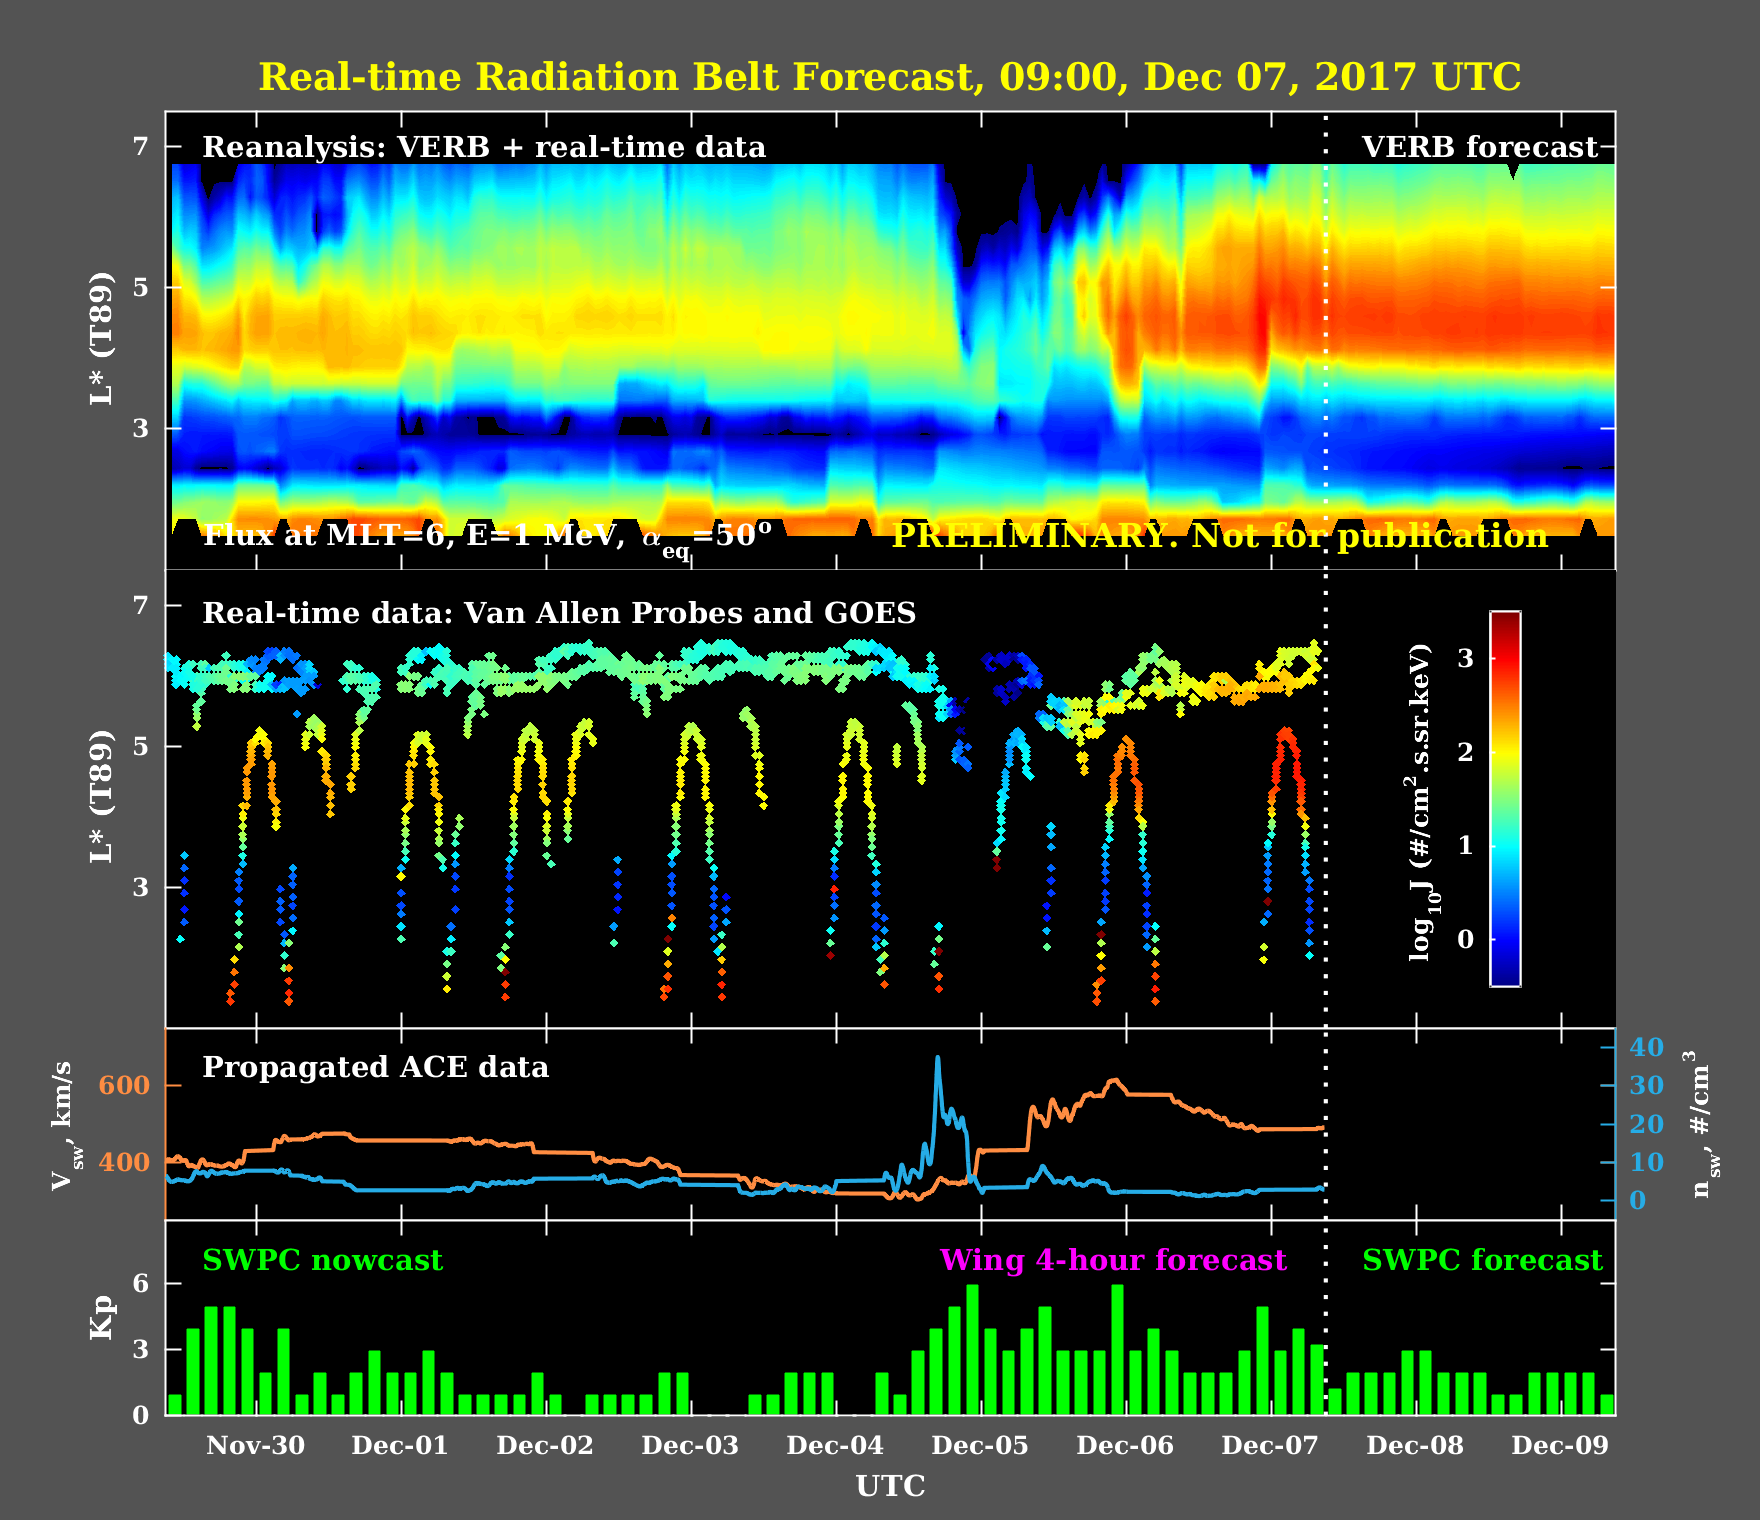
\includegraphics[width=0.5\hsize]{Forecast_UTC_latest.png} 
 %   \end{wrapfigure}
\begin{minipage}{.5\linewidth}
\begin{itemize}
    \item     Quasi-linear (diffusion) models have been very successful in understanding the dynamics of radiation belts
    \item   \textbf{Physics-based} models are gradually transitioning to real-time forecasting
    \item We believe that a \textbf{bayesian inference} approach is needed to successfully use diffusion models for forecasting\\
     See also POSTER 2534 \emph{Probabilistic Space Weather Forecasting: a Bayesian Perspective} (TODAY)
\end{itemize}
\end{minipage}
\begin{minipage}{.5\linewidth}
    \centering
    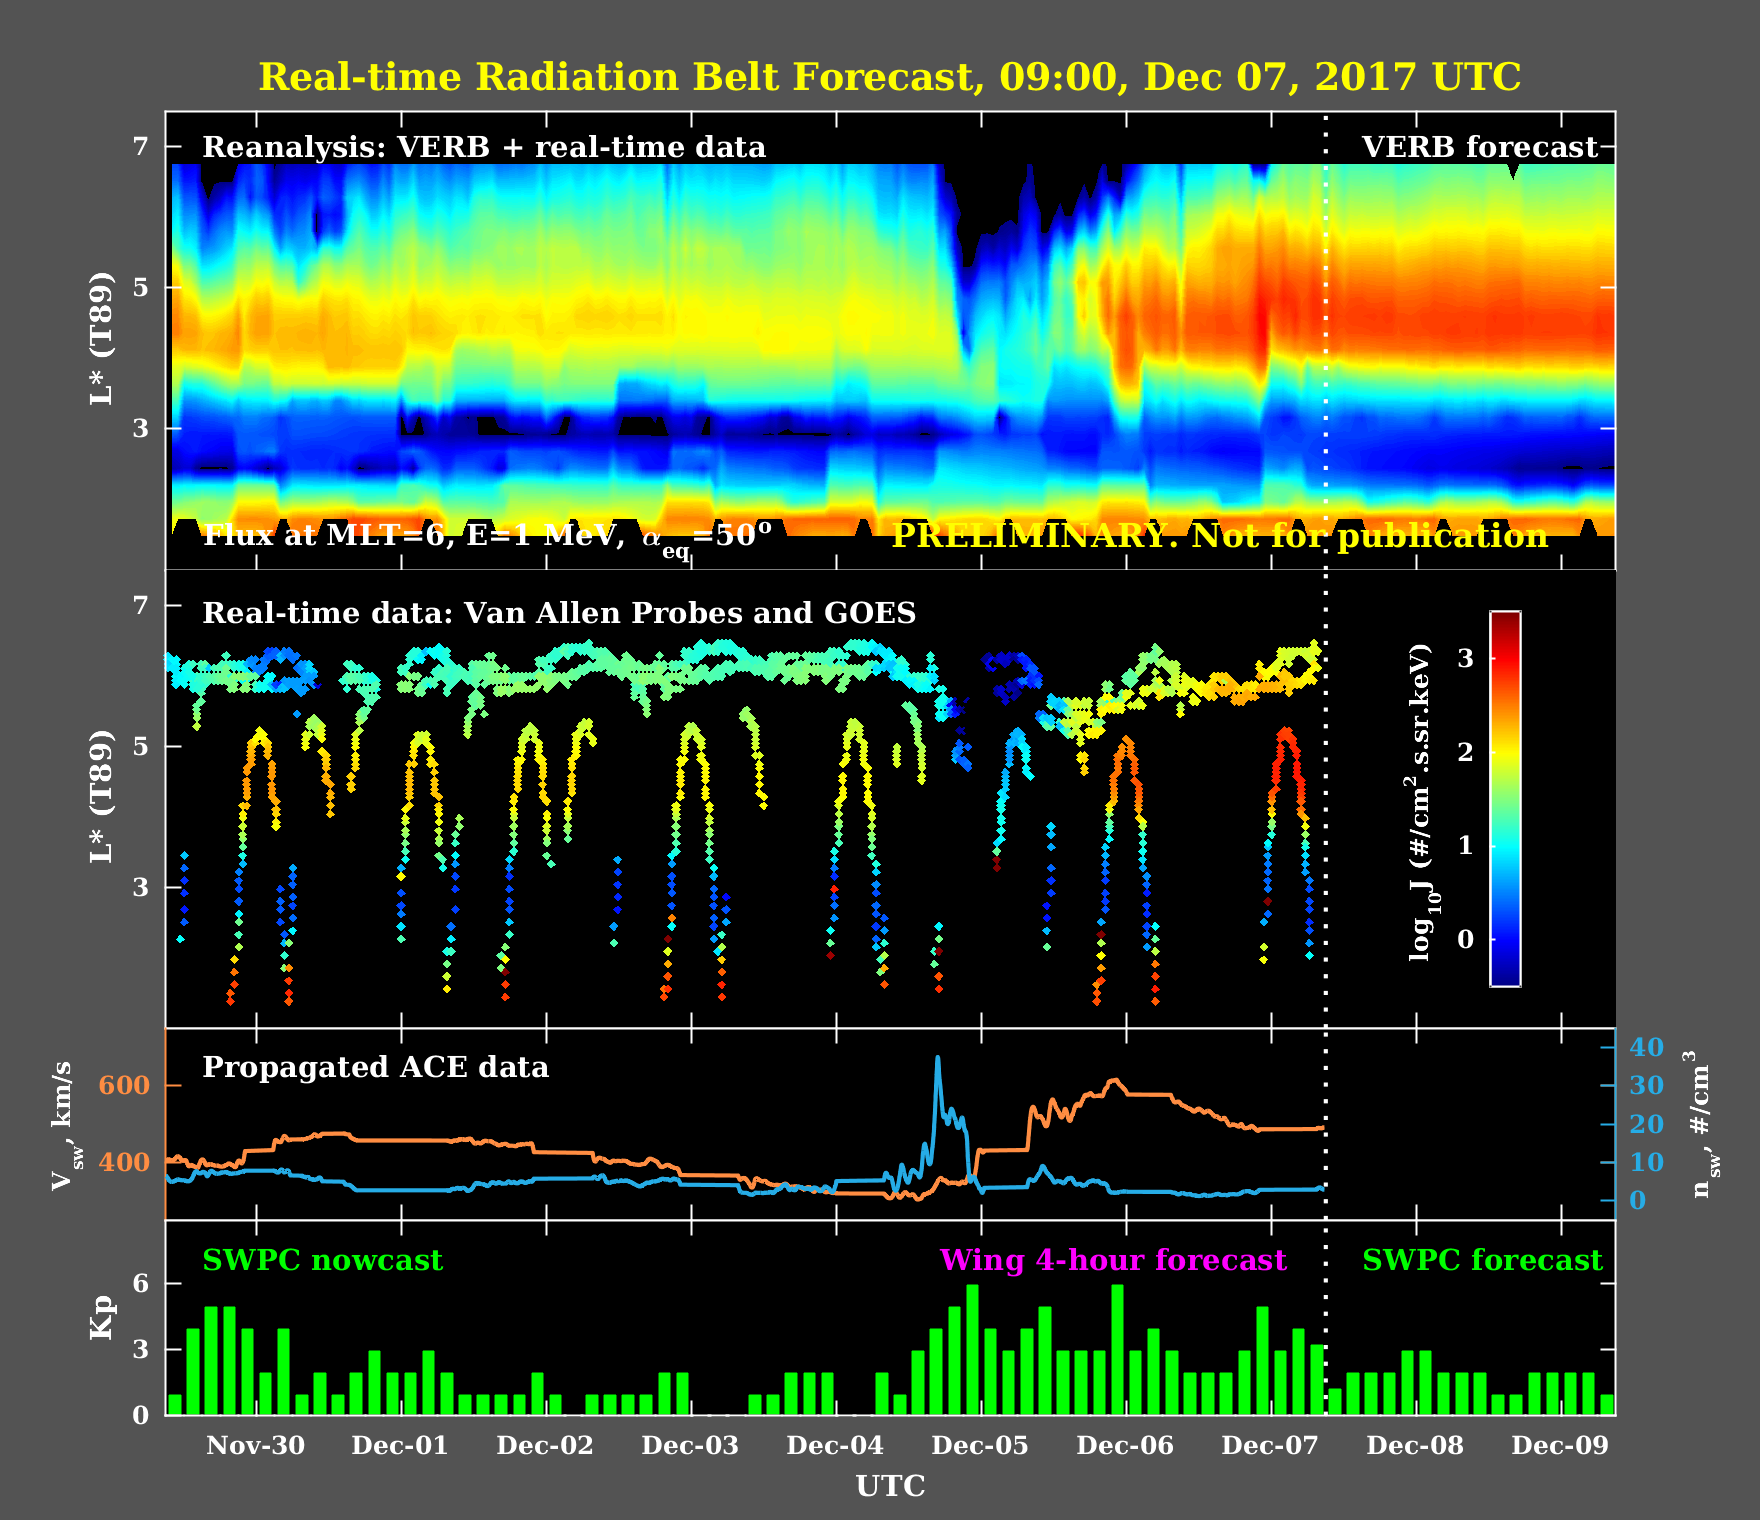
\includegraphics[width=.8\linewidth]{Forecast_UTC_latest.png}
    {\small http://rbm.epss.ucla.edu/realtime-forecast/}
   \end{minipage}
\mysection{Quasi-linear Radial Diffusion}
In this work we deal with the simplified problem of 1D radial diffusion

\begin{equation}\label{eq:raddiffusion}
  \frac{\partial{f}}{\partial{t}} = L^2 \frac{\partial}{\partial{L}}\left( \frac{D_{LL}}{L^{2}} \frac{\partial{f}}{\partial{L}} \right) - \frac{f}{\tau}+ Q
\end{equation}

\vspace{.5\baselineskip}

\begin{center}
\begin{tabular}{l l}
            \hline
            \noalign{\smallskip}
            Quantity &  Meaning \\
            \noalign{\smallskip}
            \hline
            \noalign{\smallskip}
            $f(L, t)$ & phase space density\\
            $D_{LL}(L, t)$ & diffusion coefficient\\
            $\tau(L, t) > 0$ & electron lifetime\\
            $Q(L, t)$ & injection or source term\\
            \noalign{\smallskip}
            \hline
\end{tabular}
\end{center}

\mysection{Input Parameters}

To solve the radial diffusion system in equation \ref{eq:raddiffusion}, $D_{LL}$, $\lambda=\frac{1}{\tau}$ and $Q$ need to be
specified. 

It is a common practice to parameterise the diffusion field $D_{LL}$ and loss rate $\lambda$, in terms of dependencies over space $L$ and over global geomagnetic activity $Kp$.

\begin{align}
  D_{LL}(L,t) &\sim \alpha_{\kappa} L^{\beta_{\kappa}} 10^{b_{\kappa} Kp(t)} \\
  \lambda(L, t) &\sim \alpha_{\lambda} L^{\beta_{\lambda}} 10^{b_{\lambda} Kp(t)}\\
  Q(L, t) &\sim (\alpha_{q} L^{\beta_{q}} + \gamma_{q})10^{b_{q} Kp(t)}
\end{align}


Determining values of these parameters from observations is known as the \emph{inverse problem}, this is challenging due to:

\begin{enumerate}
    \item Sparse and irregular observations
    \item Lack of knowledge about initial and boundary conditions, i.e. problem is ill-posed.
\end{enumerate}

\vfill
\columnbreak

\mysection{Methodology}


We build a surrogate model for $f$ of the form $\hat{f}(x) = \sum_{i = 1}^{d} w_{i}\varphi_{i}(x) + b$, where $\varphi_{i}(.)$ are some basis functions. 

\vspace{.5\baselineskip}

To calculate the coefficients of the surrogate model, we minimize the square error of the surrogate model which is a combination of:

\begin{enumerate}
    \item Observational error $e_{k}$
    \item Colocation error $\epsilon_{k}$, which measures how much the surrogate violates the radial diffusion PDE in equation \ref{eq:raddiffusion}.
\end{enumerate}

\begin{align}\label{eq:surrogate}
   min_{w,e,\epsilon} \ \mathcal{J}(w,e,\epsilon;\theta) &= 
   \frac{1}{2} w^{T}w + \frac{1}{2\gamma_{o}} \sum_{k = 1}^{n_{o}}{e^{2}_{k}} + \frac{1}{2\gamma_{c}} \sum_{k = 1}^{n_{c}}{\epsilon^{2}_{k}} \\
  & s.t \nonumber \\
  y_{i} & = w^{T}\varphi(x^{o}_{i}) + b + e_{i}, \ \ i = 1 \cdots n_{o} \\
  q_{i} & = w^{T}\psi(x^{c}_{i}) + \epsilon_{i}, \ \ i = 1 \cdots n_{c}
\end{align}

\mysection{Inference}

Before performing \emph{markov chain monte carlo} (MCMC) inference over the diffusion parameters, we must define the \emph{prior} and \emph{likelihood} models.

\vspace{.5\baselineskip}

\begin{center}
\begin{tabular}{lllll}
    \toprule
    \cmidrule{1-2}
    Quantity     & $\alpha$     & $\beta$ & $\gamma$ & $b$ \\
    \midrule
    $\lambda$ & $Lognormal(0, 1)$ & $Gamma(1, 1)$ & N.A & $\mathcal{N}(0, 2)$ \\
    $Q$ & $Lognormal(0, 2)$ & $Gamma(1, 1)$ & $Lognormal(0, 2)$ & $\mathcal{N}(0, 2)$ \\
    \bottomrule
\end{tabular}
\end{center}

\vspace{.5\baselineskip}

We assume a multivariate gaussian distribution for calculating the likelihood of the observations conditioned on the system parameters. The covariance between observations made at two points is assumed to decay with their space-time distance as $C(x_{i}, x_{j}) = \sigma^2 exp(-\frac{1}{2} (\frac{|l_i - l_j|^2}{s} + \frac{|t_i - t_j|}{r}))$.

\begin{equation}
\begin{bmatrix}
y_1\\ 
\vdots\\ 
y_{n_o}
\end{bmatrix} | x_1, \cdots, x_{n_o}, [\alpha, \beta, \gamma, b]_{Q, \lambda},  \sim \mathcal{N} \left(\begin{bmatrix}
\hat{f}(x_1)\\ 
\vdots\\ 
\hat{f}(x_{n_o})
\end{bmatrix}, \begin{bmatrix}
C(x_1, x_1) & \cdots  & C(x_1, x_{n_o})\\ 
\vdots & \ddots & \vdots\\ 
C(x_{n_o}, x_{n_{1}}) & \cdots  & C(x_{n_o}, x_{n_{o}})
\end{bmatrix} \right )
\end{equation}


\mysection{Experiments}

To test our inference procedure, we devise a synthetic example, we start by choosing some \emph{ground-truth} values for the parameters of $D_{LL}$, $\lambda$ \& $Q$, we fix the parameters of the diffusion coefficient and focus only on sampling from the parameters of $\lambda$ and $Q$.

\begin{center}
\begin{tabular}{lllll}
    \toprule
    \cmidrule{1-2}
    Quantity  & $\alpha$ & $\beta$ & $\gamma$ & $b$ \\
    \midrule
    $Q$ & $1$ & $0.5$ & $0.05$  & $0.45$     \\
    $D_{LL}$  & $4.731 \times 10^{-10}$ & $10$  & $0$ & $0.506$ \\
    $\lambda$ & $0.3678$ & $0.5$  & $0$ & $-0.2$ \\
    \bottomrule
\end{tabular}
\end{center}

We also choose an initial condition $f(t = 0)$ and a synthetic Kp profile and generate phase space density data using a diffusion solver.

\begin{center}
\begin{tabular}{c c}
    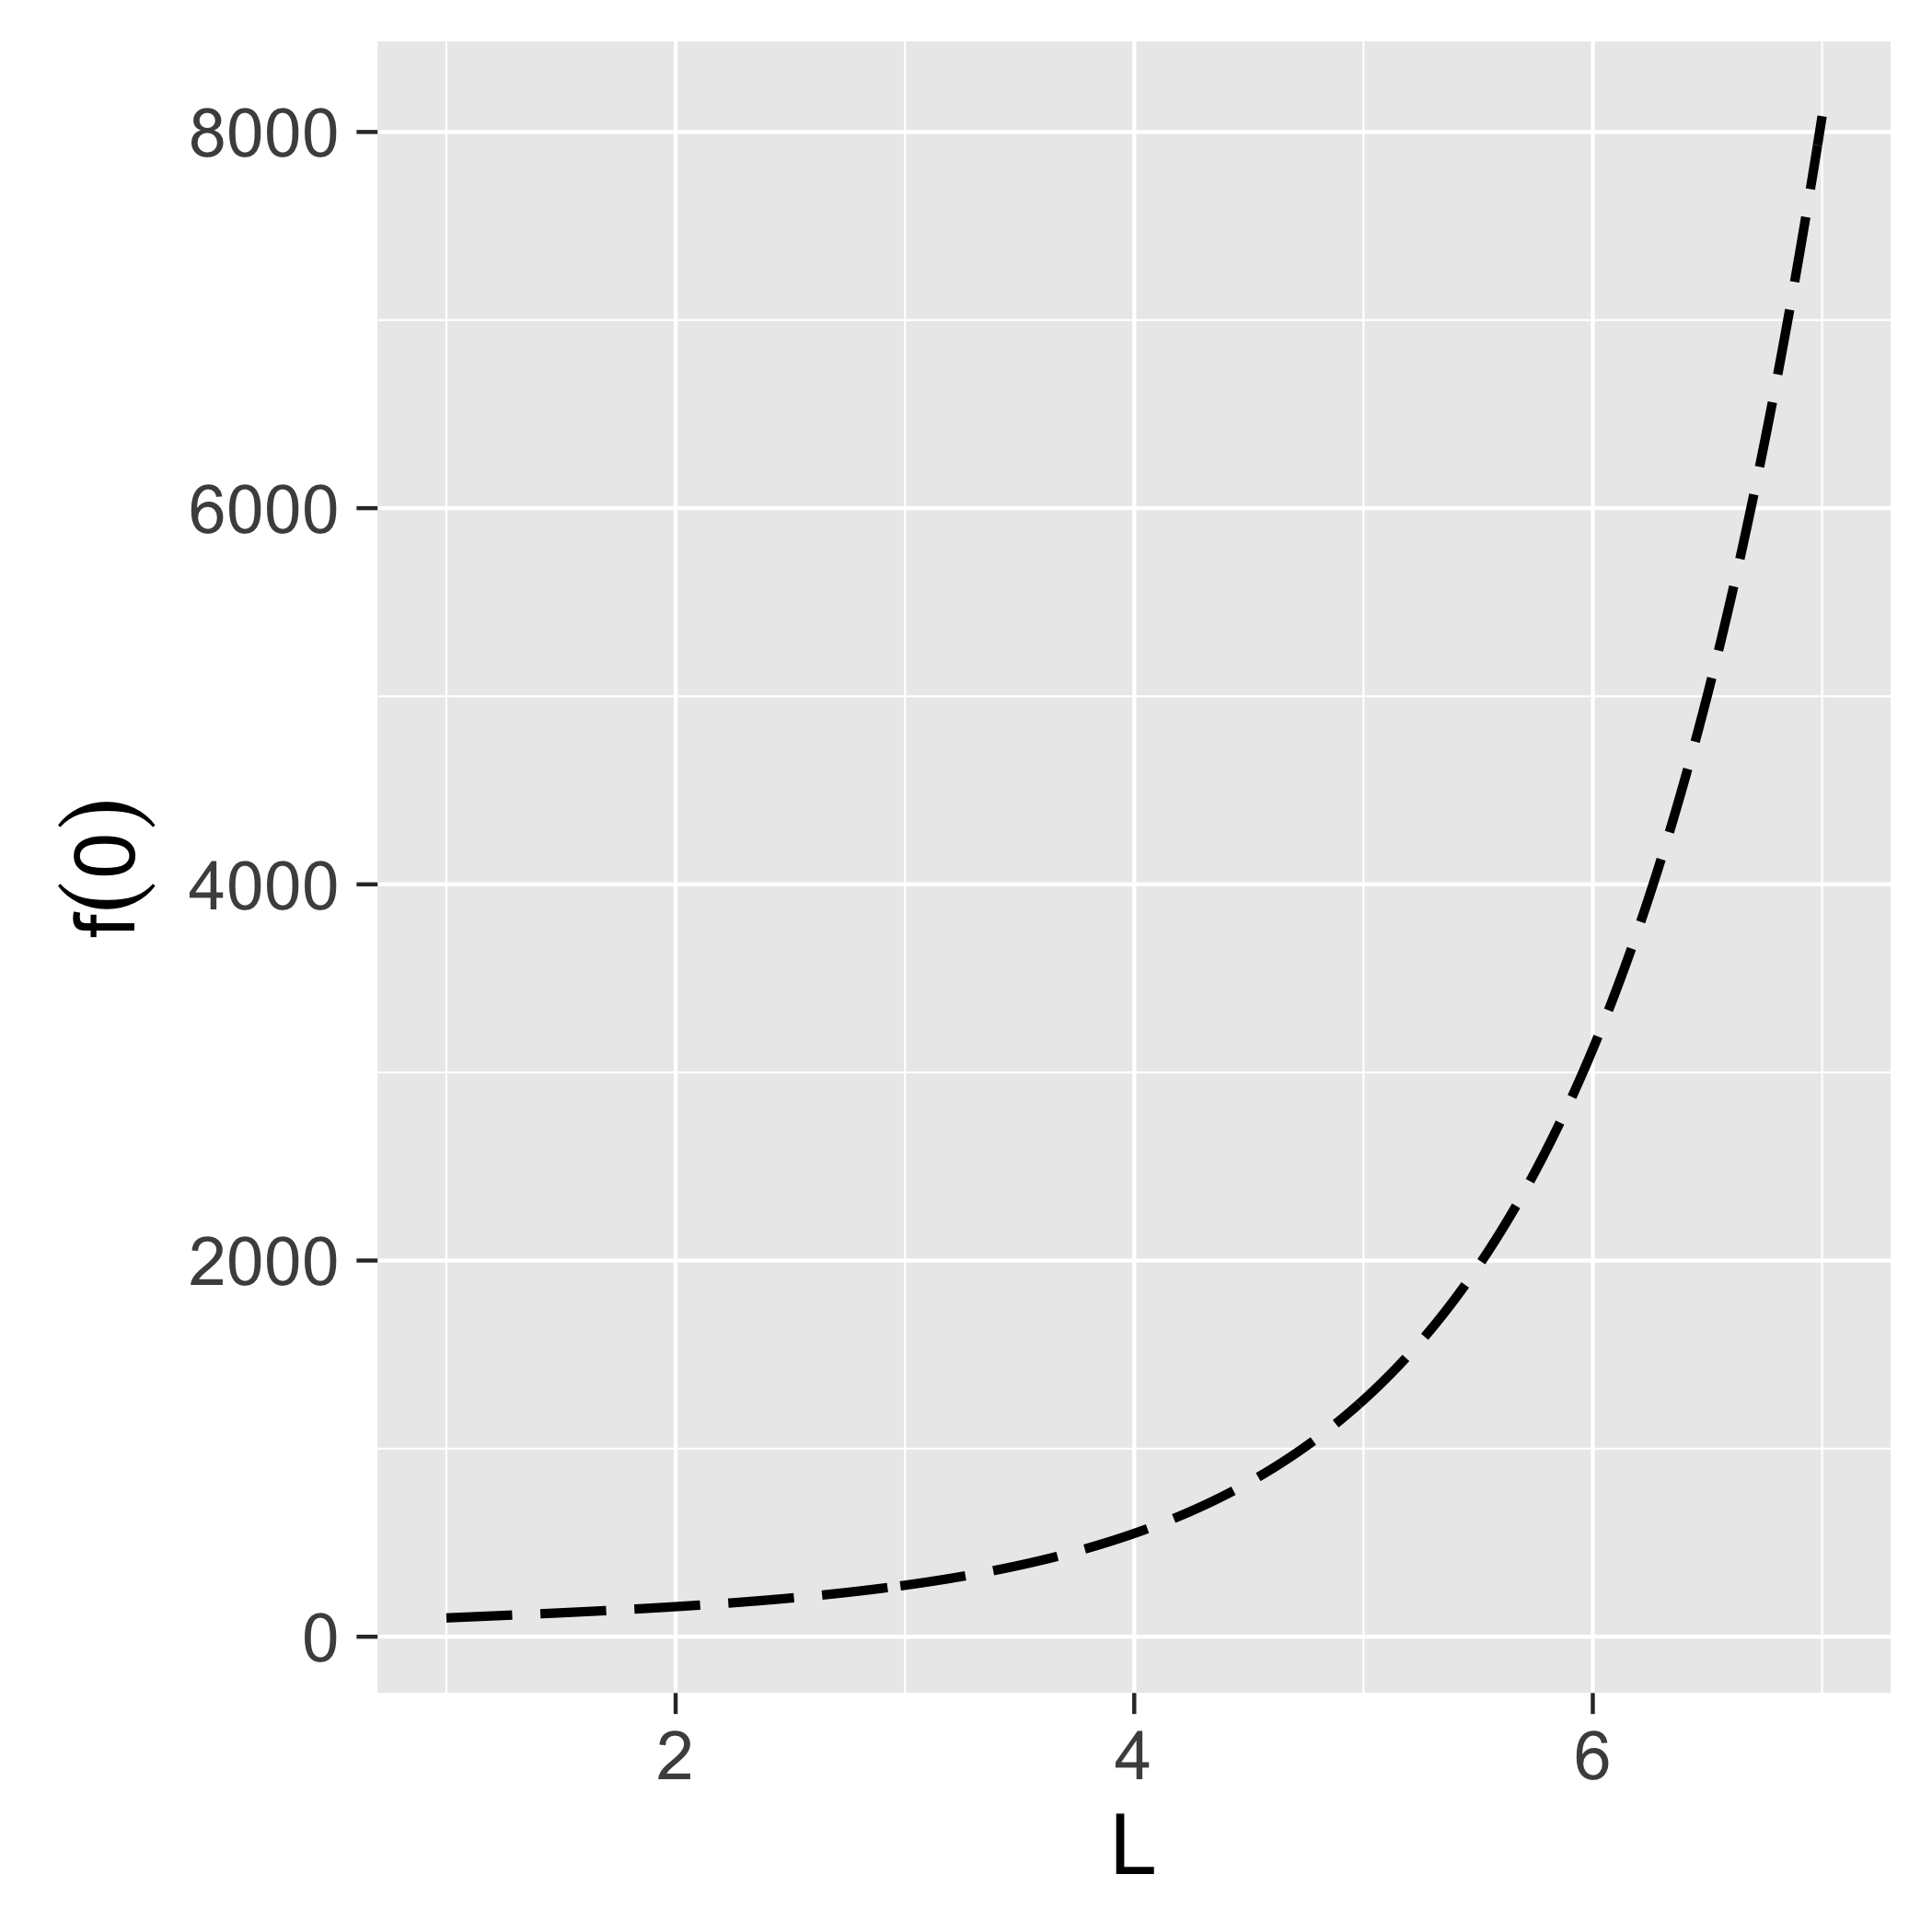
\includegraphics[width=0.45\linewidth]{initial_psd} & 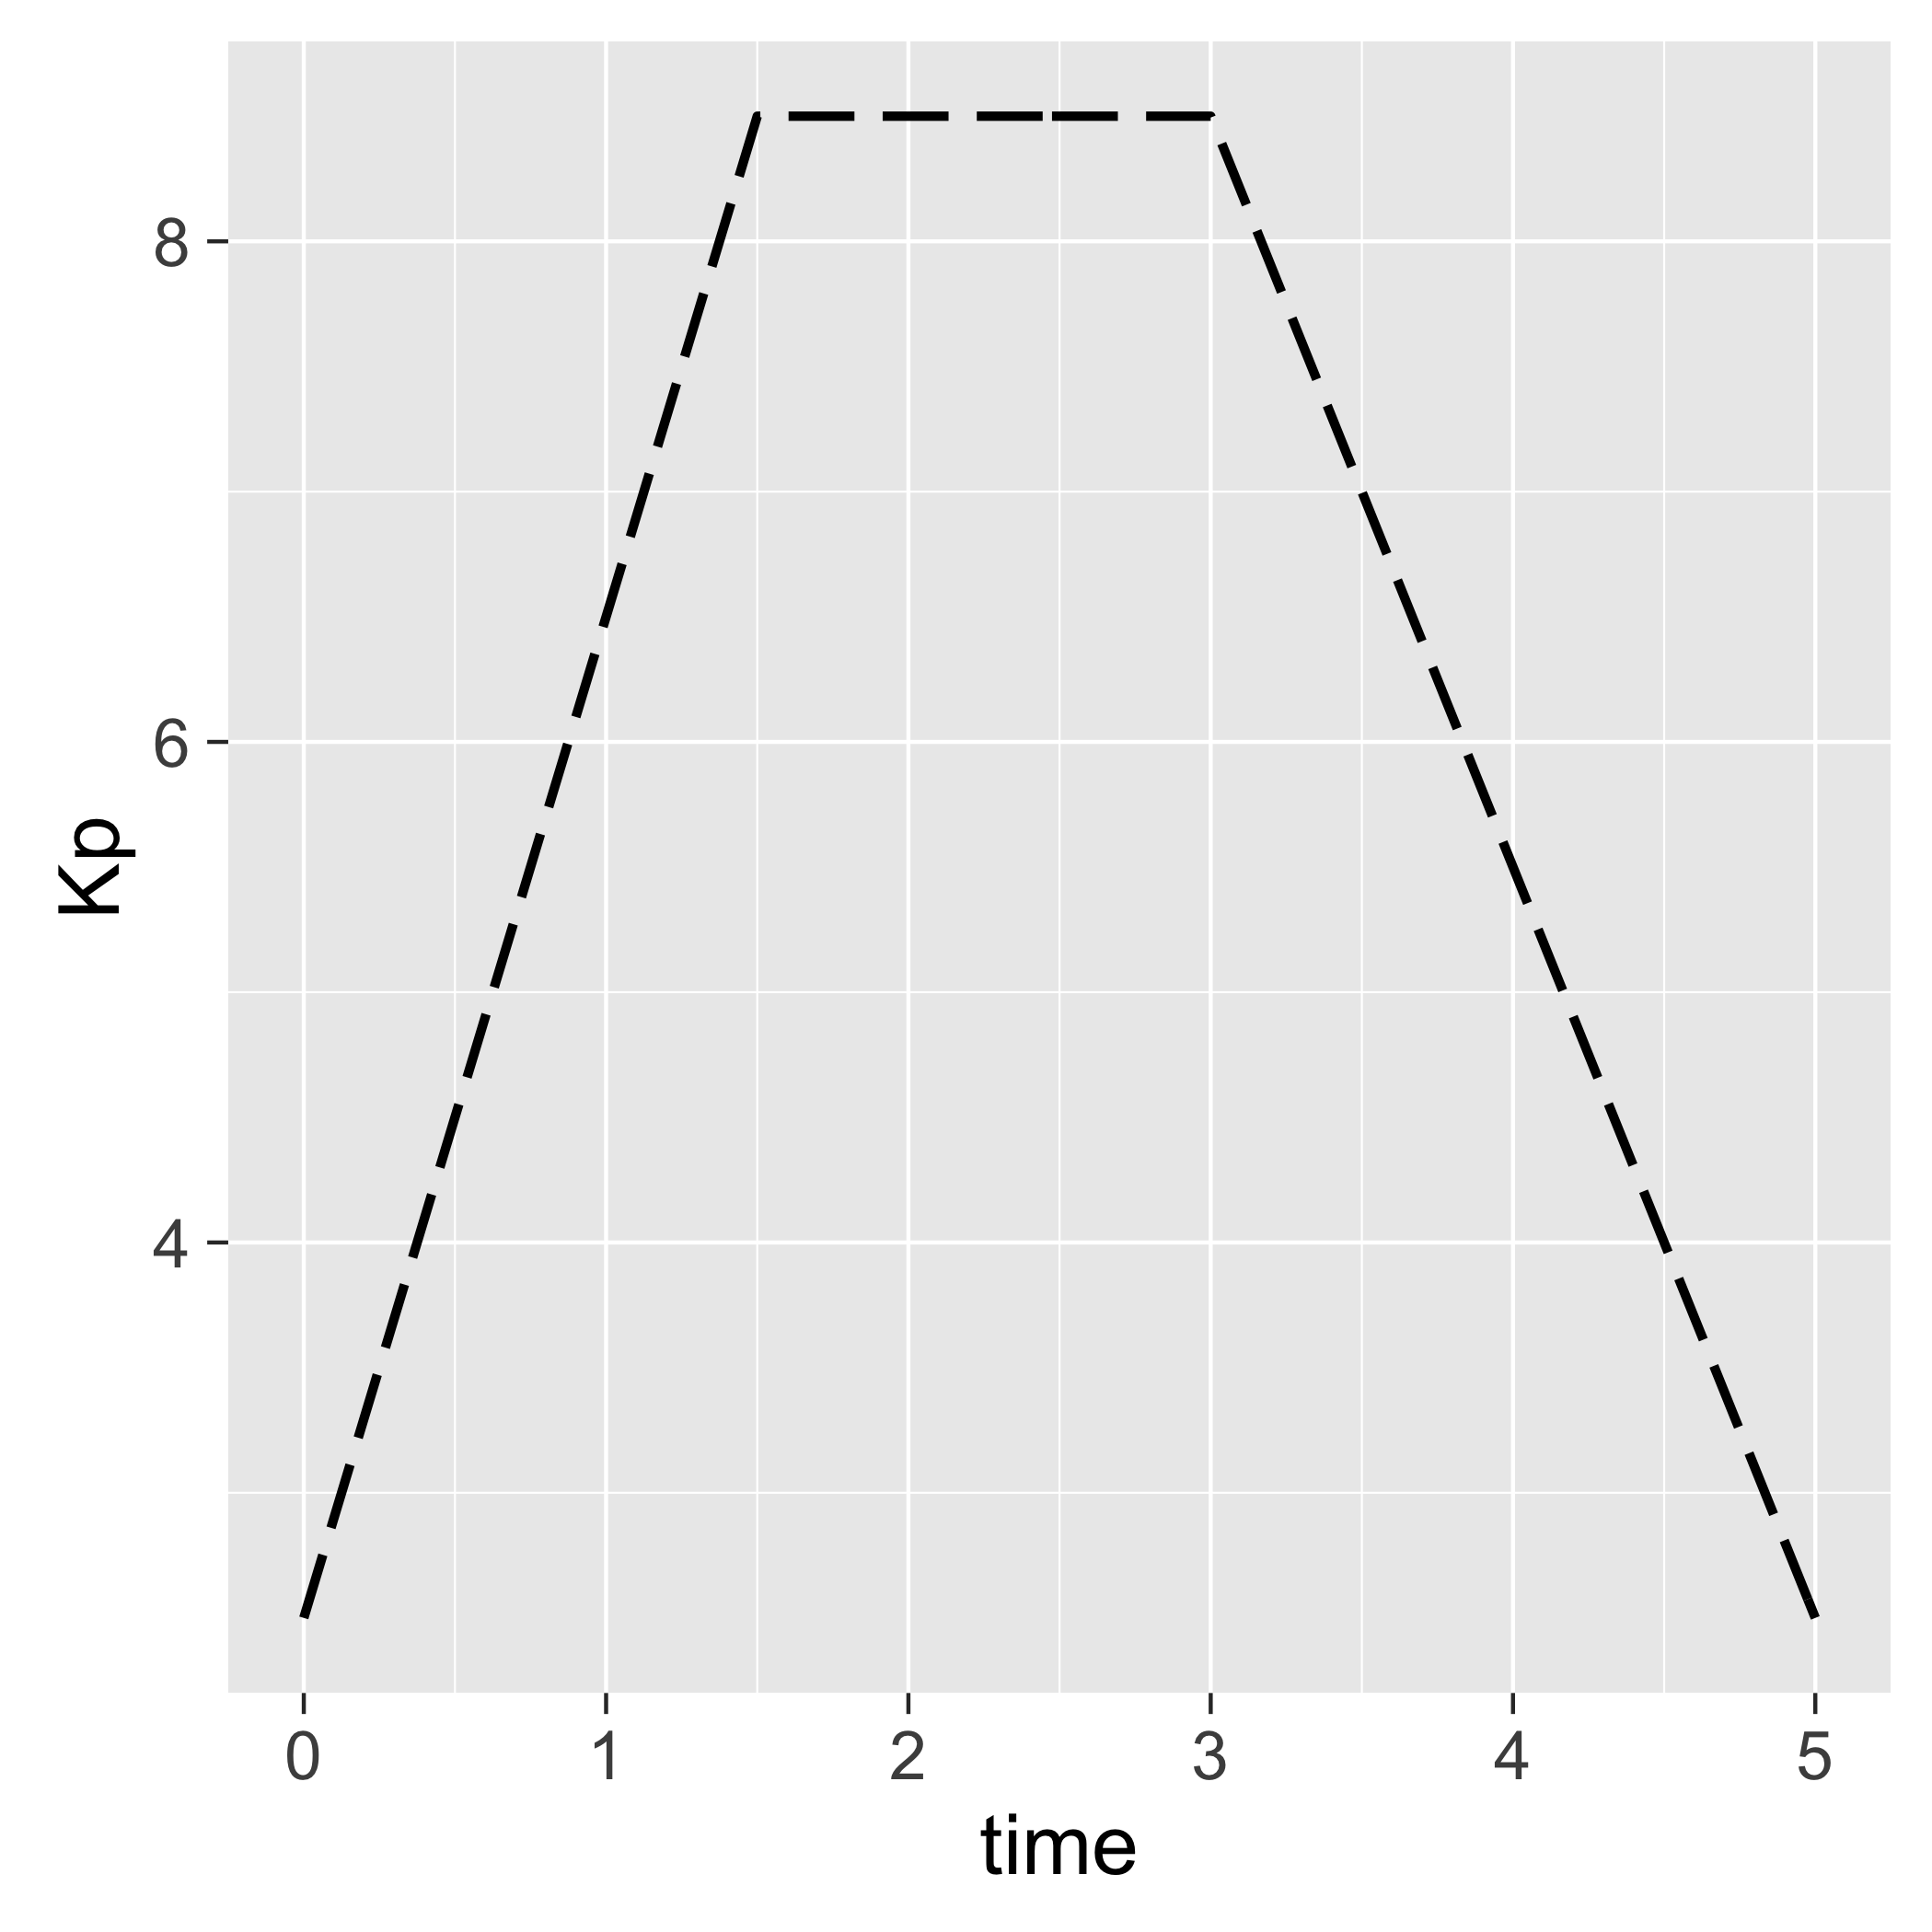
\includegraphics[width=0.45\linewidth]{kp_profile}\\
    {\small Phase space density profile at $t = 0$} & {\small Kp profile for a \emph{synthetic} geomagnetic storm}
\end{tabular}
\end{center}


\begin{center}
\begin{tabular}{c c}
    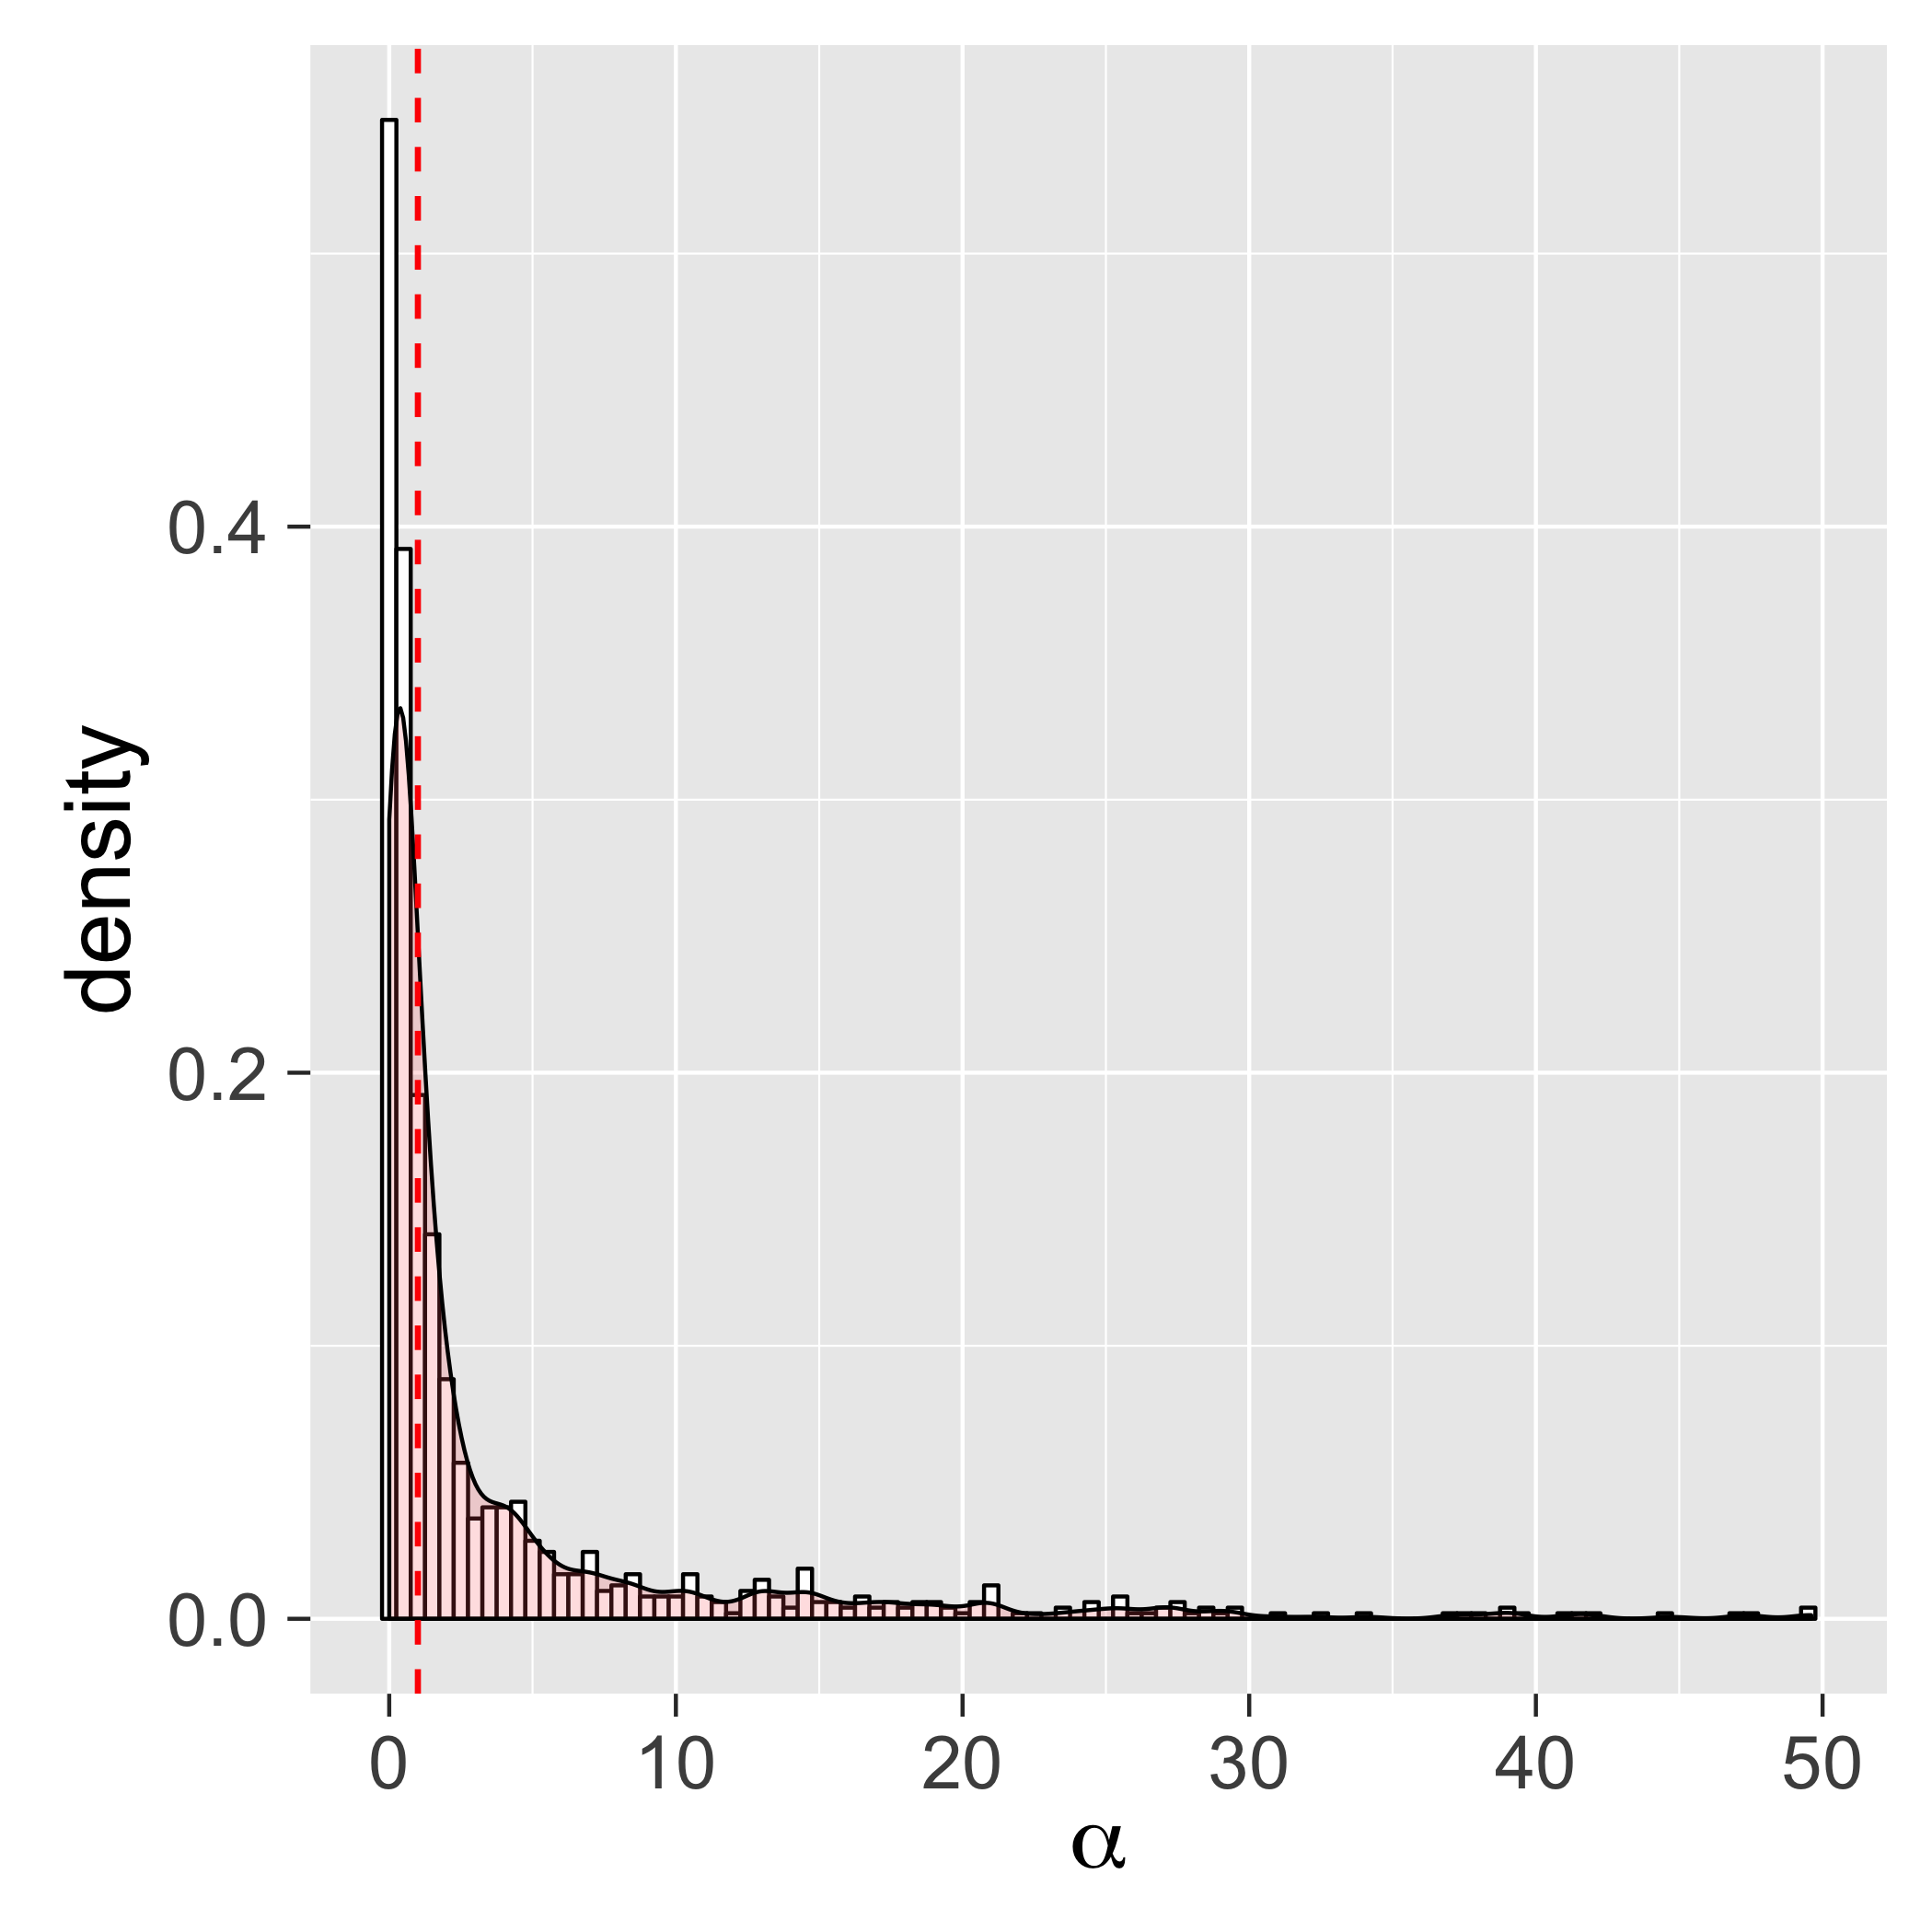
\includegraphics[width=0.45\linewidth]{histogram_Q_alpha_posterior} & 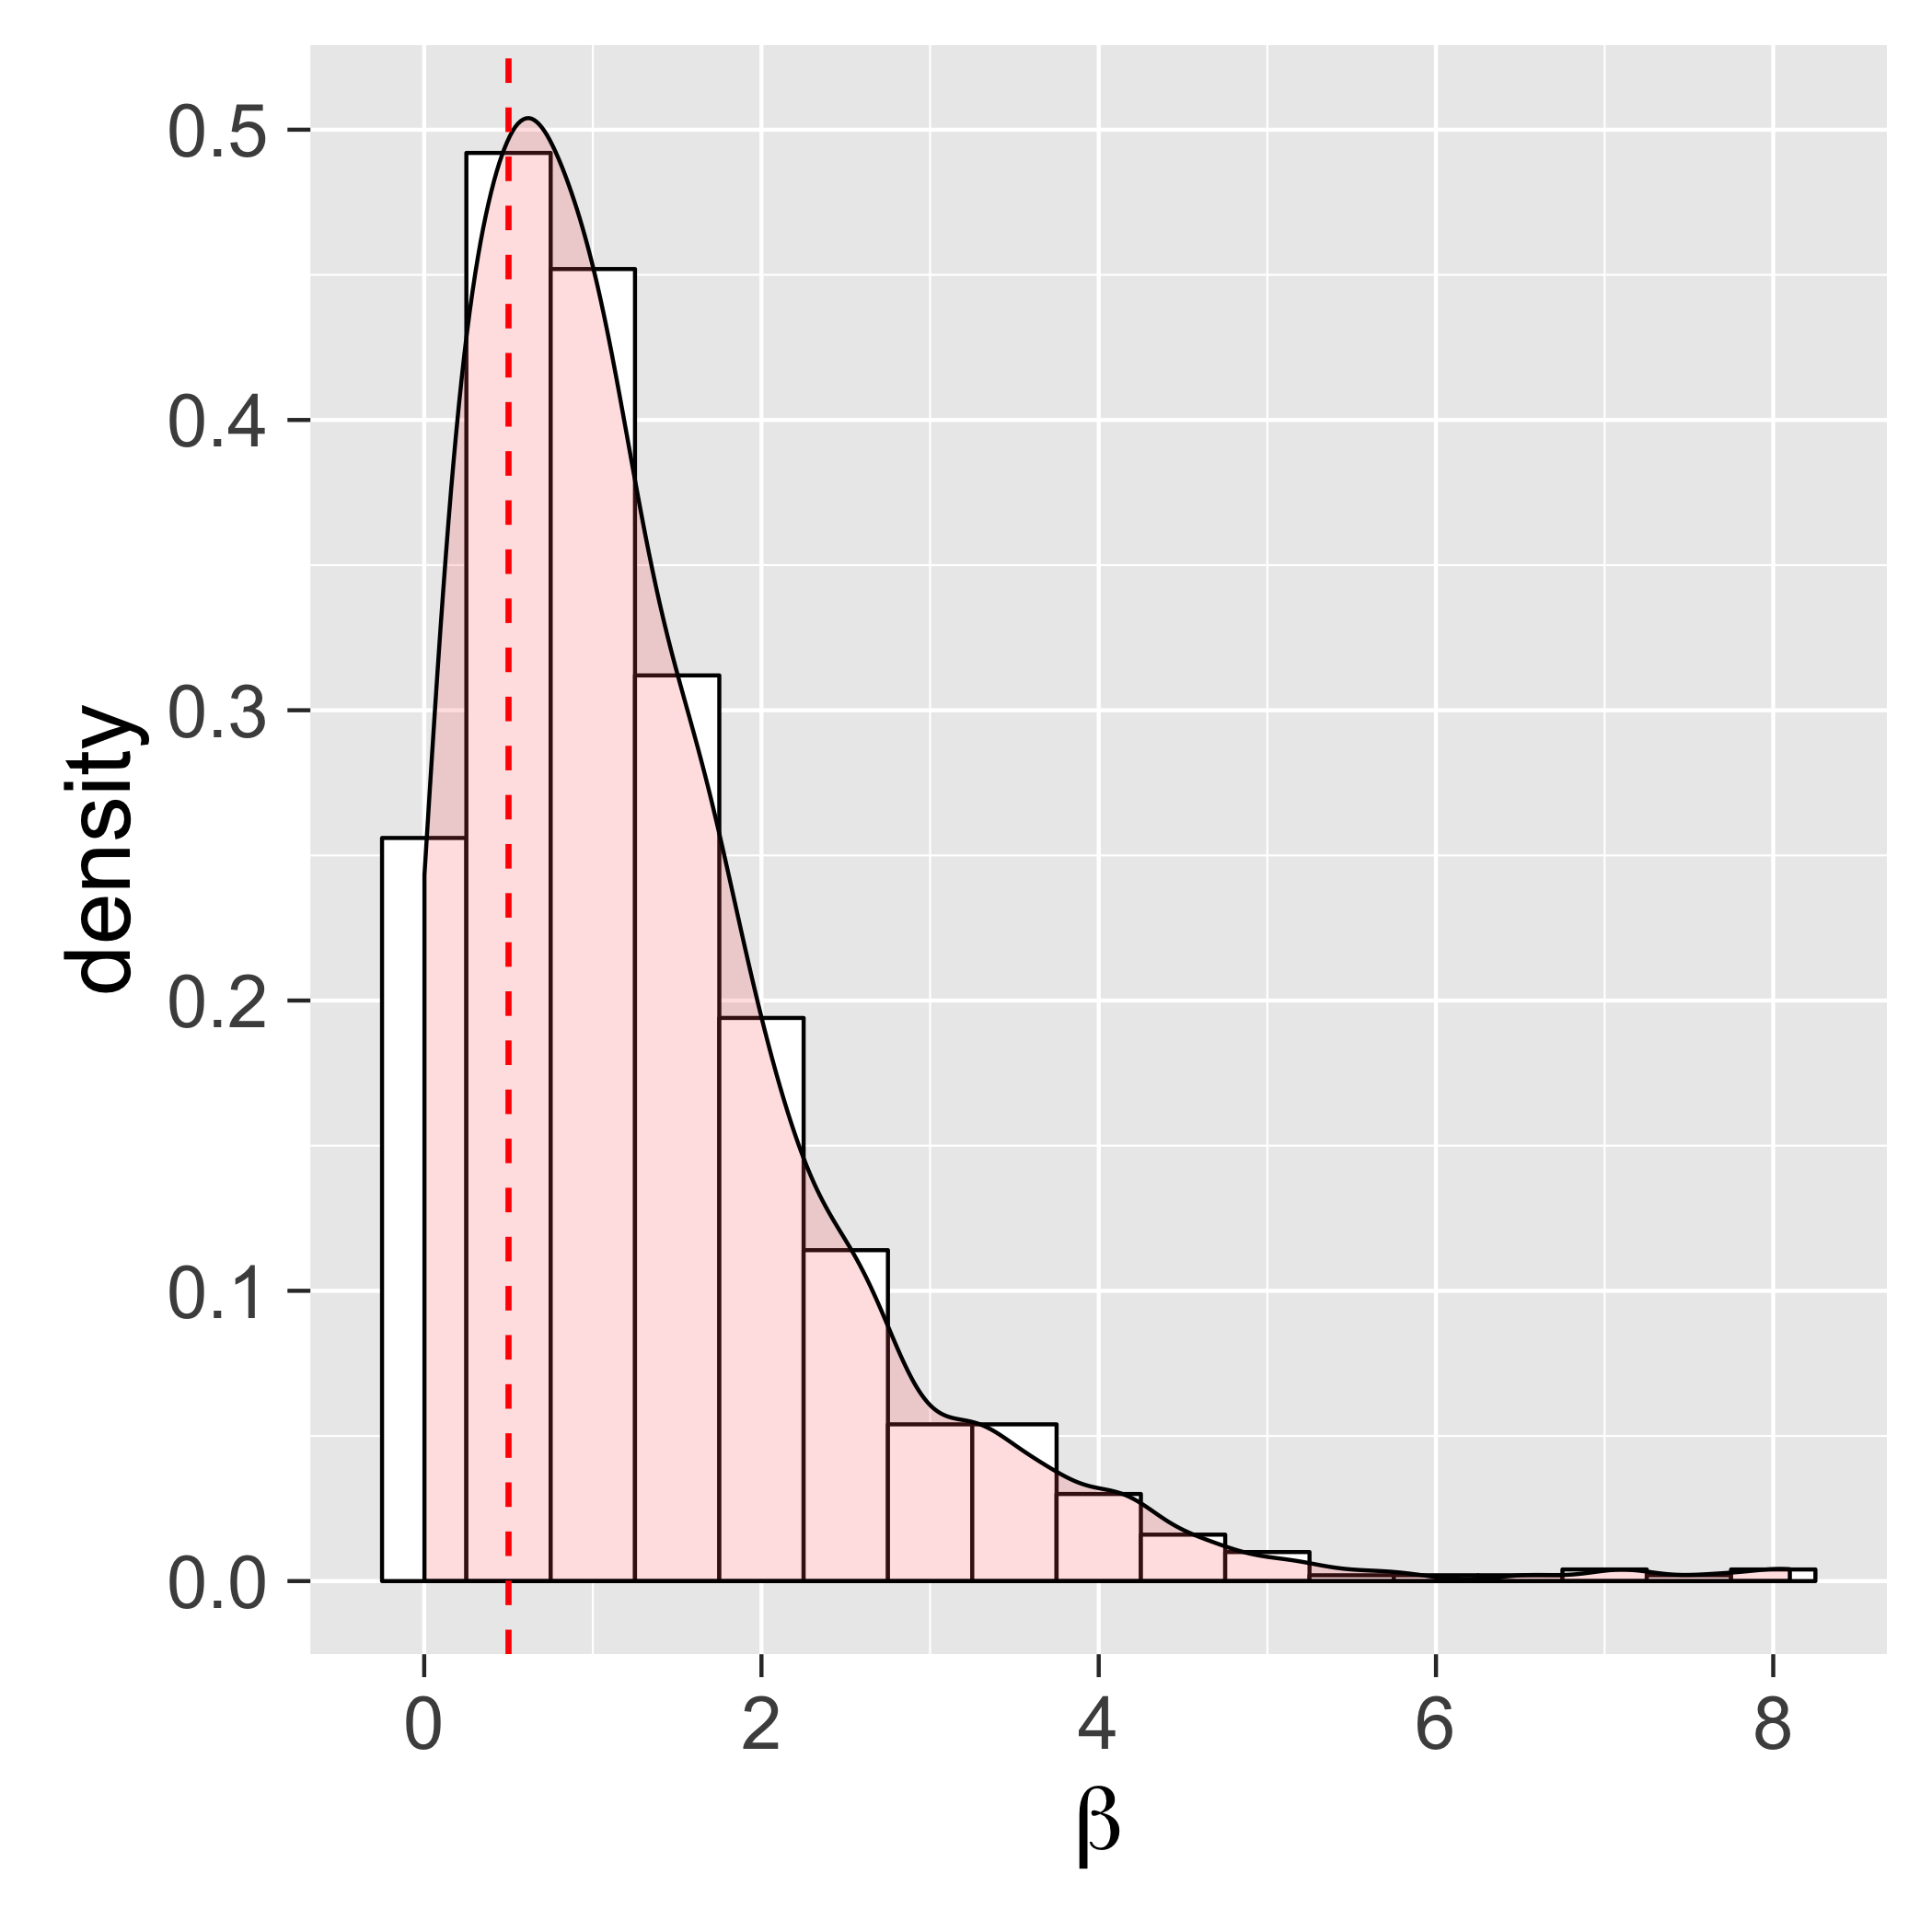
\includegraphics[width=0.45\linewidth]{histogram_Q_beta_posterior}\\
\end{tabular}
{\small Posterior samples for parameters $\alpha$ and $\beta$ of $Q$}
\end{center}

\vspace{\baselineskip}

\begin{center}
\begin{tabular}{c c}
    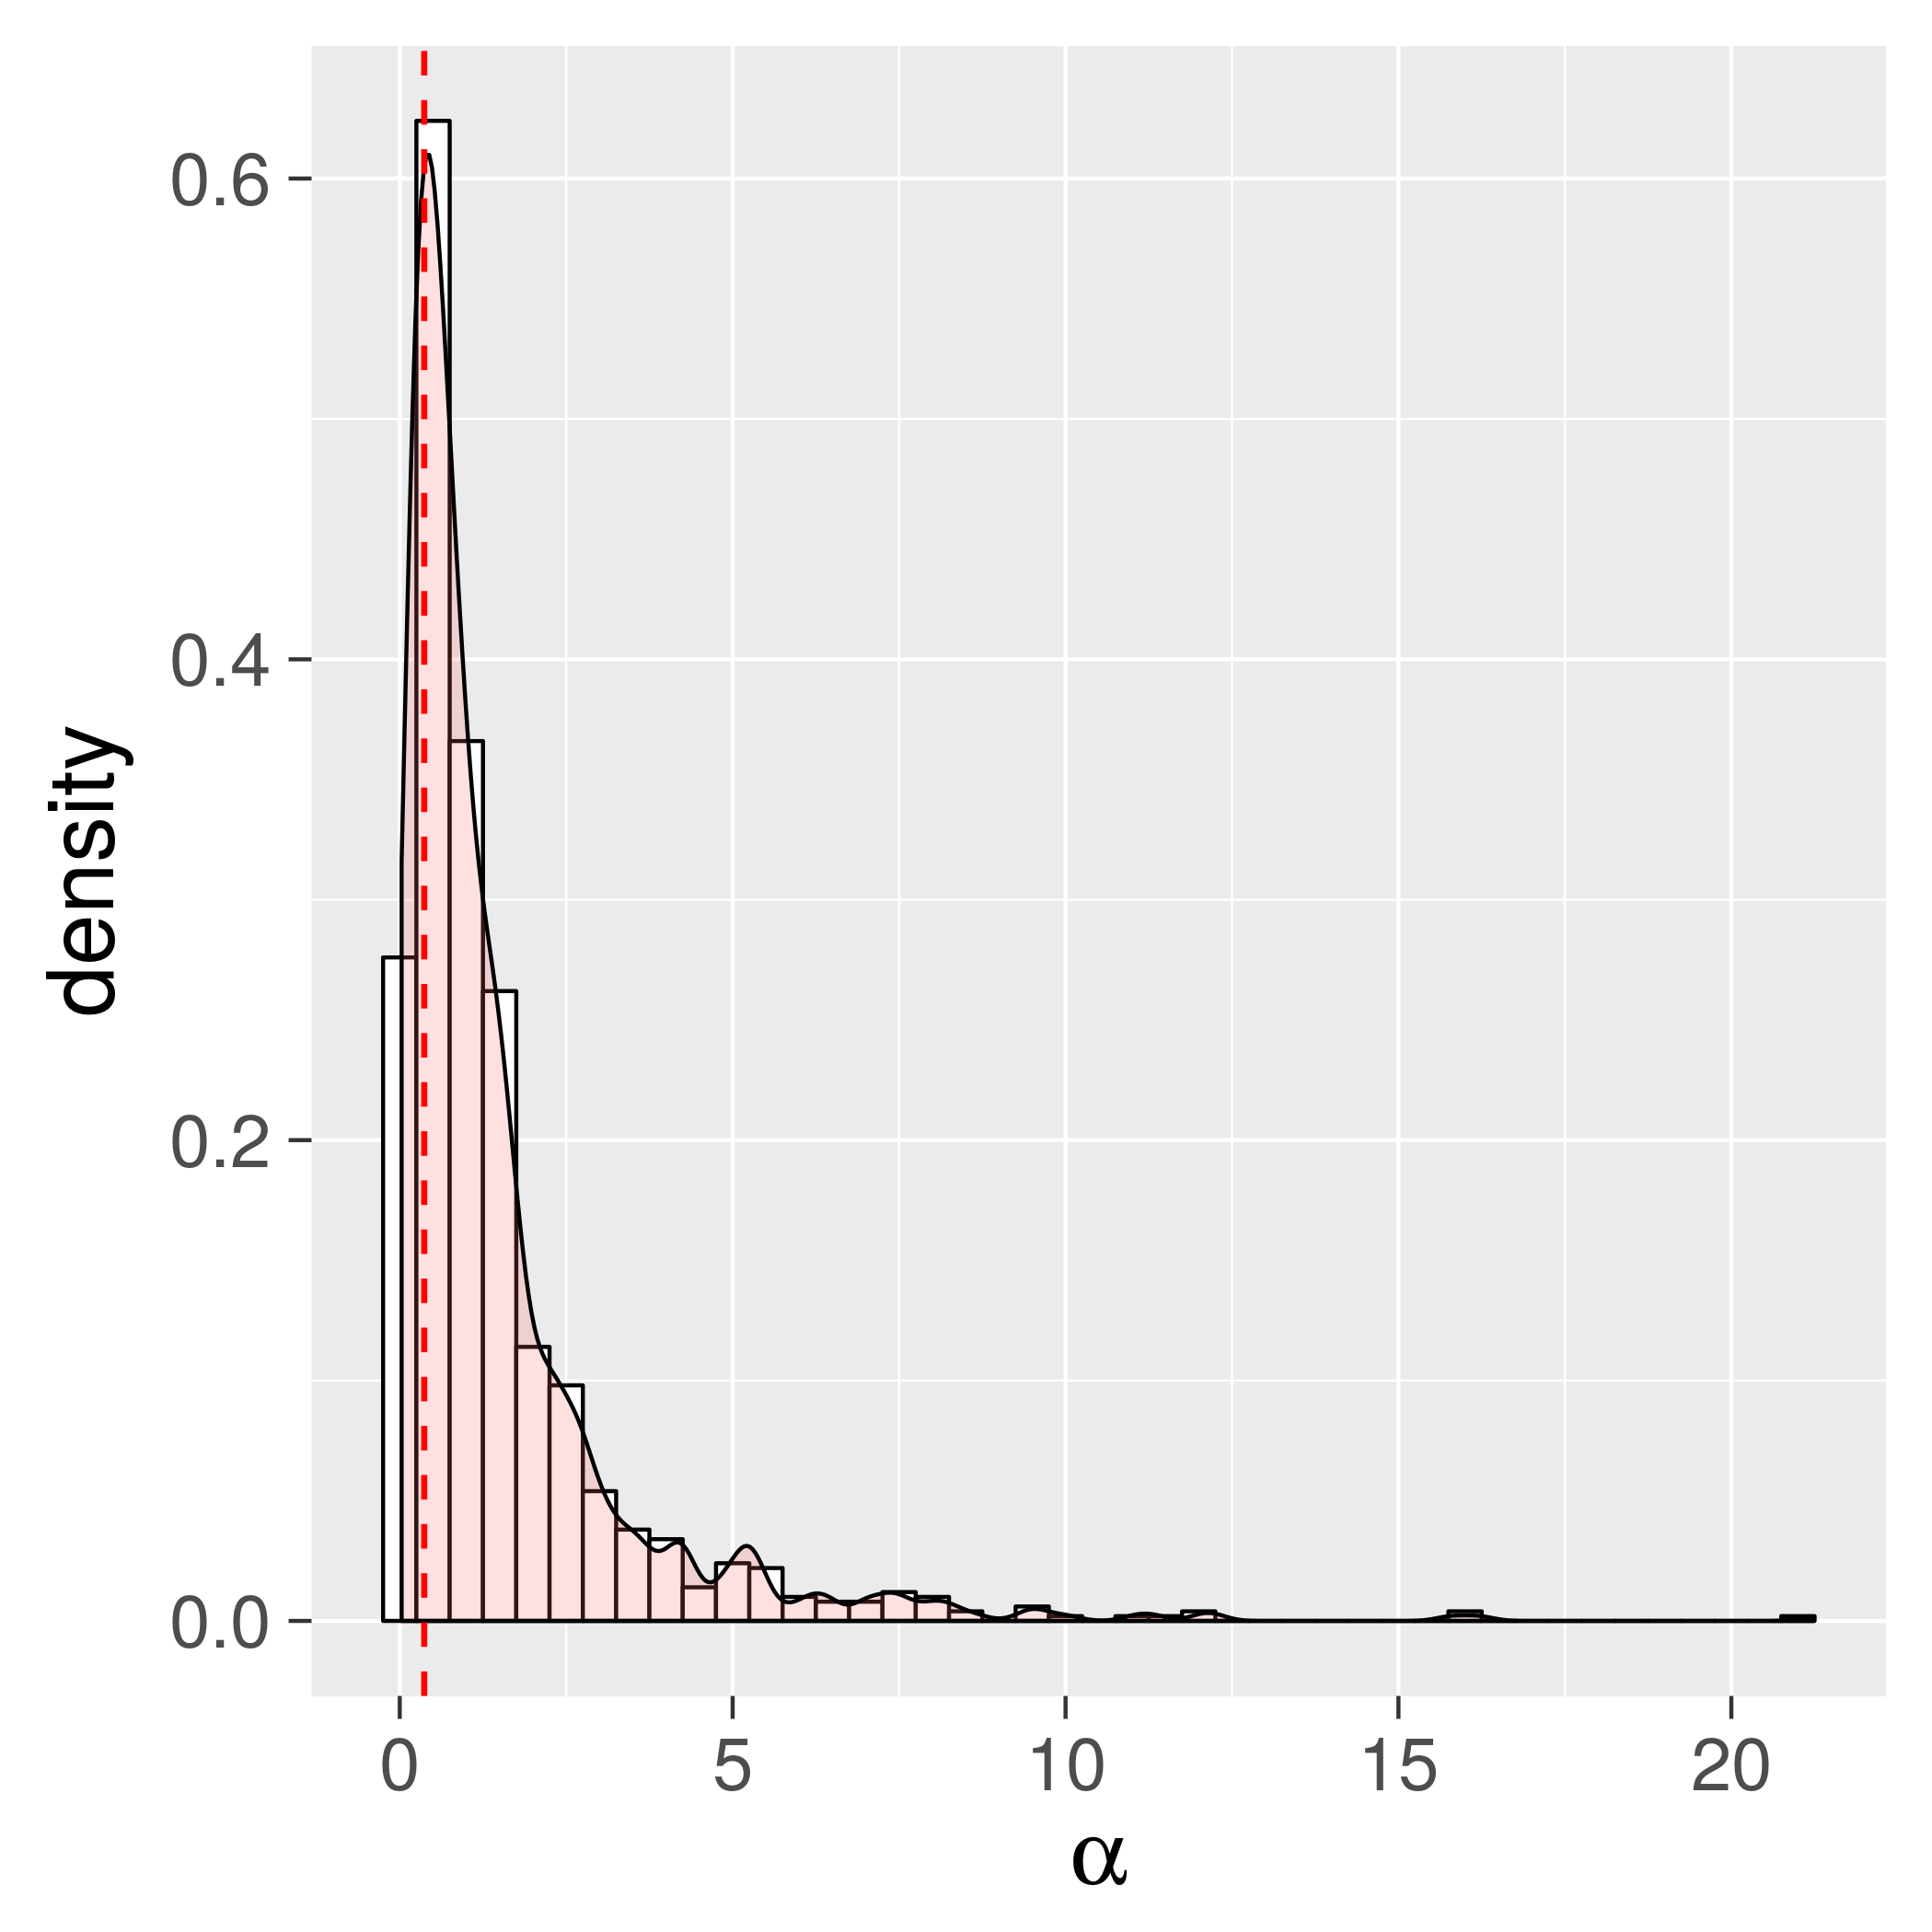
\includegraphics[width=0.45\linewidth]{histogram_tau_alpha_posterior} & 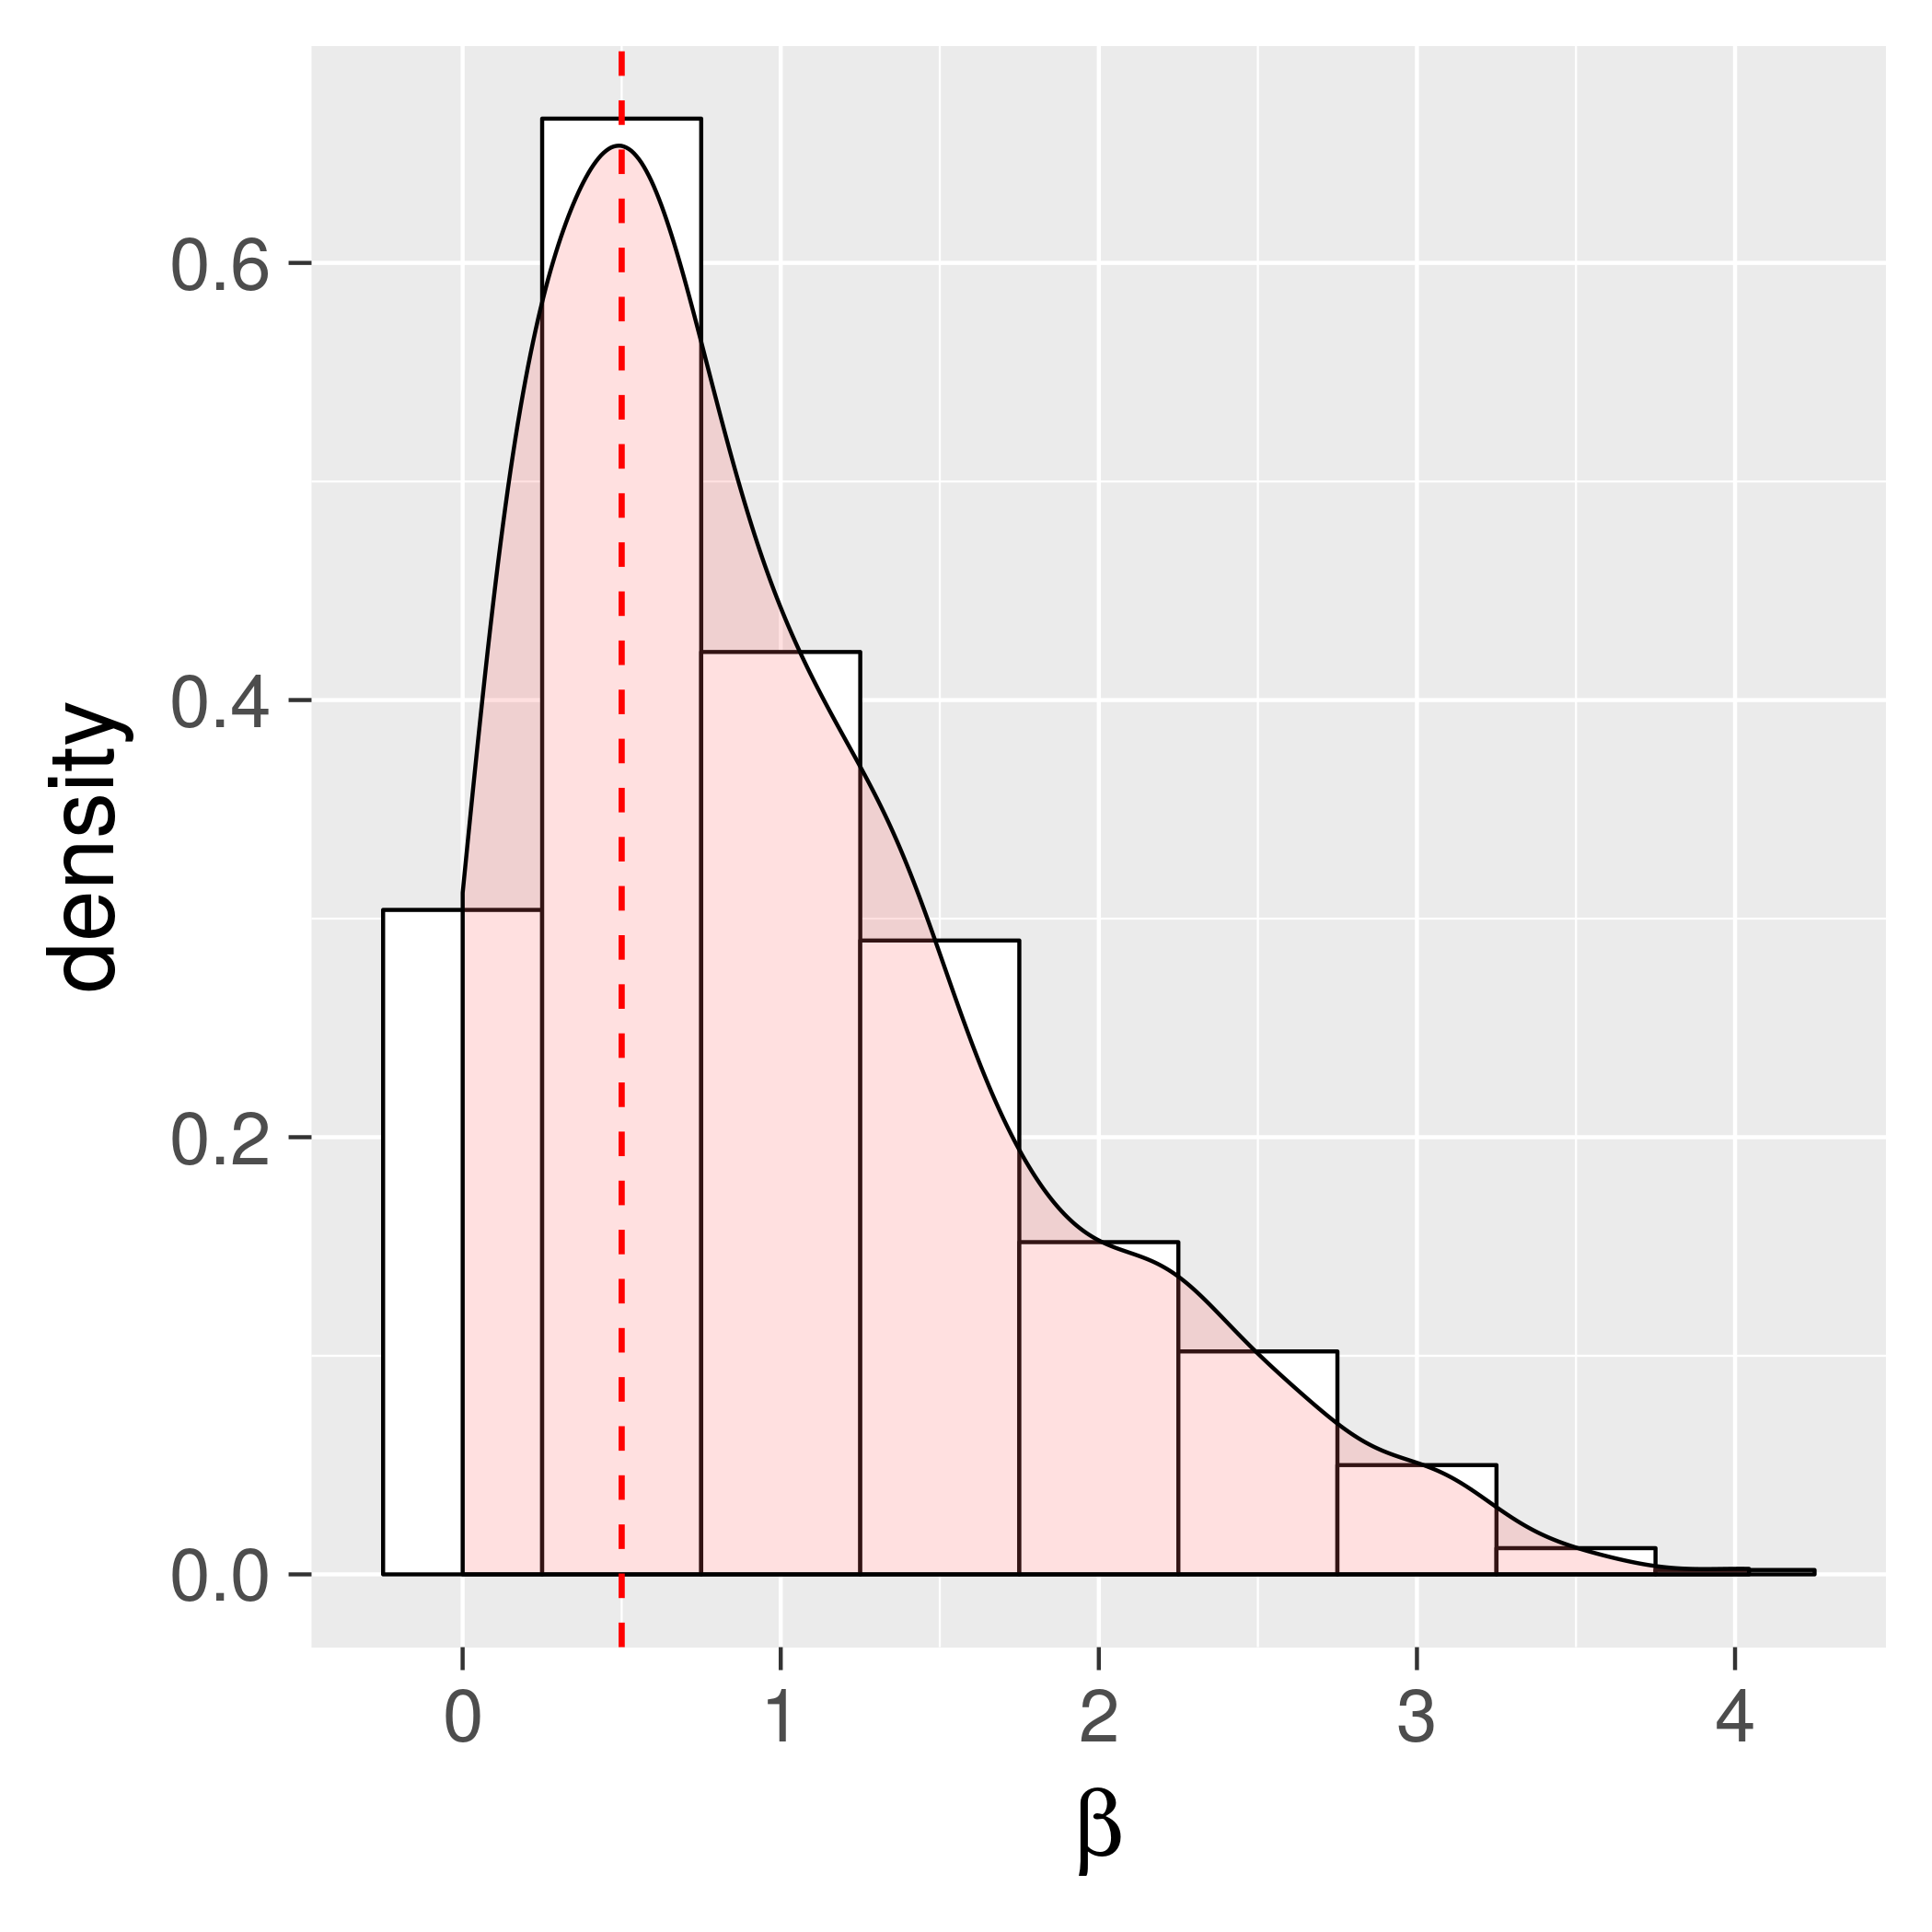
\includegraphics[width=0.45\linewidth]{histogram_tau_beta_posterior}\\
\end{tabular}
{\small Posterior samples for parameters $\alpha$ and $\beta$ of $Q$}
\end{center}


\vspace{\baselineskip}
\mysection{Conclusions}
\begin{enumerate}
    \item The marginal posterior distributions of each parameter have high probability density near the ground truth, and that they are heavy tailed because there are often large regions of the parameter space which produce similar solutions for $f$. 
    \item The strength of the proposed method is the ability to quantify the uncertainty in diffusion parameters from a set of irregularly spaced observations.
    \item The method can be extended to 3-dimensional quasi-linear diffusion problems.\\
\end{enumerate}
\vspace{.5\baselineskip}


\end{multicols}

\end{poster}

\end{document}
